\section{Scope of the assignment}
\subsection{Our network}
The target network belongs to the fictitious \textbf{ACME co.}, which requires a series of tools and security checks to be implemented in the hosts of the network itself.\\
All the hosts can be reached through a \textbf{VPN}. Though the network is quite large and comprehends a number of more than ten hosts, in this paper we will focus only on a specific subnet, that is the one where the security measures are to be implemented according to the scope of this assignment.\\
Thus, from now on we will not refer to the topology of the whole network, but only on the topology of the \textbf{Clients network}.

\subsection{Our scope}
The aforementioned \textbf{Clients network} is pictured in \textbf{Figure 1}, and is assigned the corresponding IP address \textbf{100.100.2.0/24}.\\

\begin{figure}[htpb]
\centering
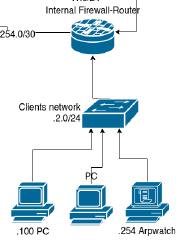
\includegraphics[width=0.3\textwidth]{clientsNetwork.png}
\caption[a]{The \textbf{Clients network}, scope of the assignment.}\label{fig:1}
\end{figure}

The scope of the assignment is to enable the \textbf{DHCP service} on the \textit{Internal Firewall-Router}, in order to provide the clients of the target network with dynamic IPv4 addresses. Furthermore, the clients should be protected against \textbf{link-local attacks} by implementing security measures and tools on the \textbf{Arpwatch} machine with IP address \textbf{100.100.2.254}.

\subsection{Goals}
How do we plan to achieve the goals of this assignment?
General ideas.
